\documentclass{article}
\usepackage[a4paper]{geometry}
\geometry{
  a4paper,
  top=40mm,
}
\usepackage[utf8]{inputenc}
\usepackage[english]{babel}
\usepackage{changepage}

\usepackage{graphicx}
\usepackage{wrapfig}
\usepackage{caption}
\captionsetup[figure]{labelformat=empty}

\usepackage{hyperref}
\hypersetup{
  colorlinks=true,
  linkcolor=blue,
  filecolor=magenta,
  urlcolor=cyan,
}

\usepackage{algpseudocode}
\usepackage{minted}
\usepackage{algorithm}


\usepackage{fontspec}
	\newfontfamily\mathfont{CMU Serif}
\newfontfamily\monospace{Roboto Mono}

\usepackage{amsmath, amssymb, amsfonts, amsthm, fouriernc, mathtools}
\usepackage{microtype}

\usepackage[svgnames]{xcolor}
\definecolor{lightgrey}{rgb}{0.5,0.5,0.5}
\definecolor{grey}{rgb}{0.25,0.25,0.25}
\newcommand{\blackb}{\color{Black} \usefont{OT1}{lmss}{m}{n}}
\newcommand{\lightgreyb}{\color{lightgrey} \usefont{OT1}{lmss}{m}{n}}
\usepackage{tikz}
\usepackage{caption}

\let\bold\textbf
\newcommand\comb[2][^n]{\prescript{#1\mkern-0.5mu}{}C_{#2}}

\usepackage{titlesec}
\usepackage{sectsty}
\sectionfont{\color{lightgrey}}
\subsectionfont{\color{lightgrey}}
\subsubsectionfont{\color{lightgrey}}

\renewcommand\thesection{\Roman{section}}
\renewcommand\thesubsection{\arabic{section}.\arabic{subsection}}
\renewcommand\thesubsubsection{\arabic{section}.\arabic{subsection}.\arabic{subsubsection}}

\counterwithin*{equation}{section}

\newcommand{\mysection}{
\titleformat{\section} [runin] {\usefont{OT1}{lmss}{b}{n}\color{lightgrey}}
{\thesection} {3pt} {} }

\renewcommand{\theequation}{\arabic{section}.\arabic{equation}}

\usepackage{etoolbox}
\makeatletter
\patchcmd{\@Aboxed}{\boxed{#1#2}}{\colorbox{black!15}{$#1#2$}}{}{}
\patchcmd{\@boxed}{\boxed{#1#2}}{\colorbox{black!15}{$#1#2$}}{}{}
\makeatother

\title{\vspace{80mm}\lightgreyb CS345: Algorithms II \\
\lightgreyb Assignment $1$ Solution}
\author{Ayush Bansal \\
Roll No. 160177}
\date{\today}

\newtheorem{theorem}{Theorem}
\newtheorem{corollary}{Corollary}[theorem]
\newtheorem{conjecture}{Conjecture}
\newtheorem{lemma}{Lemma}[section]
\newtheorem{claim}{Claim}[section]
\newenvironment{solution}
  {\begin{proof}[Solution]}
  {\end{proof}}
\AfterEndEnvironment{theorem}{\noindent\ignorespaces}
\renewcommand\thelemma{\arabic{section}.\arabic{lemma}}
\renewcommand\theclaim{\arabic{section}.\arabic{claim}}

\newenvironment{myenv}{\begin{adjustwidth}{1cm}{}}{\end{adjustwidth}}

\begin{document}
\clearpage\maketitle
\thispagestyle{empty}
\newpage
\setcounter{page}{1}
\section{Problem 7(b)}{
  \subsection{Problem Statement}{
    We are given a sequence $N$ made up of $n$ digits. We can perform exchange operations on the digits of this sequence and the list of allowed exchange operations (by position in the sequence) is given to us in the form of a set $E$, $E$ is a set of some pair of integers from the set $0,1,\dots,n-1$. One exchange operation corresponds to swapping of $i^{th}$ and $j^{th}$ digit in $N$ where $\{i,j\} \in E$. \newline
    I have to design an algorithm to compute the shortest sequence of exchange operations which transforms $N$ into the largest achievable number (as an $n$-digit number).
  }
  \subsection{Brief Outline of Solution}{
    So, think of this as a graph problem whose vertex set will be a set of $n$-digit numbers which will the possible permutations of the original sequence $N$ we can get by applying operations from exchange set $E$.
    The edge-set of the above graph will be the exchange operations which leads from one permutation to another. \newline
		Finally, I will use the \bold{BFS} algorithm on this graph to find the vertex with max value and the shortest path leading up to it.
  }
  \subsection{Data Structures}{
    Firstly, I will define a structure called exchange which will contain 2 integers from the set $0,1,\dots,n-1$ denoting the position corresponding to the exchange operation to be done.
    \begin{minted}
			[
			framesep=2mm,
			baselinestretch=1.2,
			bgcolor=LightGray,
			fontsize=\footnotesize,
			linenos
			]
			{c}
typedef struct Exchange {
  tuple e;
} exchange;
		\end{minted}
    Secondly, lets look at the node structure, it will consist of the value of the node, it will a string (since sequence of digits can be large and thus, integer won't be able to hold it). It will also contain a tuple value which basically is the representation of an exchange operation, this exchange operation will give us the original number that this number was generated from.
    \begin{minted}
			[
			framesep=2mm,
			baselinestretch=1.2,
			bgcolor=LightGray,
			fontsize=\footnotesize,
			linenos
			]
			{c}
typedef struct Node {
  string value;
} node;
		\end{minted}
    Thirdly, there will be a hash table named \bold{swaps} whose keys will be nodes and the values will be the exchange tuple that led to the creation of that node. \newline
    Next, since I am going to perform a BFS operation, I will be creating a hash table named \bold{status} which will have nodes as keys and the values of the table will be one of the three which are \bold{visited}, \bold{currently-visiting}. \newline
    Finally, there will be a stack data structure used for reverse-traversal from destination vertex to initial vertex to print the exchange operations in ascending order (from initial vertex to final).
  }
	\subsection{Algorithm}{
		I will do a \bold{BFS} on the graph, but wait where is the graph, the graph will be created as the BFS algorithm is executed. I will take the initial sequence as the initial vertex and then apply each possible exchange operation from the set $E$ to get a new vertex from this one. \newline
    Firstly creating the function for swapping digits and giving a new node.
    \begin{algorithm}
    \caption{Swap digits to generate new vertex}
    \begin{algorithmic}[1]
      \Procedure{swapDigits}{$v$, $e$}\Comment{Takes initial vertex and exchange tuple}
        \State $v_{new}\gets$new-node()
        \State $v_{new}.value\gets$Swap($v.value, e$)\Comment{this function will give final string after swapping}
        \State \Return{$v_{new}$}
      \EndProcedure
    \end{algorithmic}
    \end{algorithm}
    \begin{algorithm}
      \caption{Generating largest value sequence in minimum number of swaps}
      \begin{algorithmic}[1]
        \Procedure{printPath}{$N$, $E$}\Comment{Takes original sequence and exchange operations set}
          \State $v_0\gets$New-Node()\Comment{by default value and e in new-node are both \bold{NULL}}
          \State $v_0.value\gets N$
          \State $Max\gets v_0$\Comment{Keeping track of max number}
          \State status[$v_0$]$\gets$ currently-visiting
          \State Queue$\gets$ New-Queue()
          \State Enqueue($v_0$,Queue)
          \While{Queue is not empty}
            \State $u\gets$ Dequeue(Queue)
            \ForAll{$ex\in E$}\Comment{Get new vertex by exchange operations}
              \State $v\gets$swapDigits(u,e)\Comment{Generate a new vertex}
              \If{status[$v$] is \bold{NULL}}\Comment{Key not found in status table}
                \State status[$v$]$\gets$ currently-visiting
                \State swaps[$v$]$\gets ex$\Comment{Exchange used to get this vertex} 
                \If{$v.value > Max.value$}\Comment{Comparison is created especially for strings}
                  \State $Max\gets v$
                \EndIf
                \State Enqueue($v$,Queue)
              \EndIf
            \EndFor
          \State status[$u$]$\gets$ visited
          \EndWhile
          \State stack$\gets$New-Stack()\Comment{Building stack to contain exchanges}
          \State $cur\gets Max$
          \While{$cur.value \neq v_0.value$}
            \State Push($stack$, swaps[$cur$])
            \State $cur\gets$swapDigits($cur$, swaps[$cur$])\Comment{Getting the previous Vertex}
          \EndWhile
          \While{stack is not empty}\Comment{Printing the final sequence of exchanges}
            \State $e\gets$Pop(stack)
            \State Print(e)
          \EndWhile
        \EndProcedure
      \end{algorithmic}
    \end{algorithm}
  }
  \subsection{Example}{
    For the example lets take $N = 3528$ and $E = \{(0,1), (1,2)\}$. \newline
    So, number of digits will be equal to $4$, the \bold{BFS} tree for this example: \newline

    \begin{figure}[H]
    \centering
    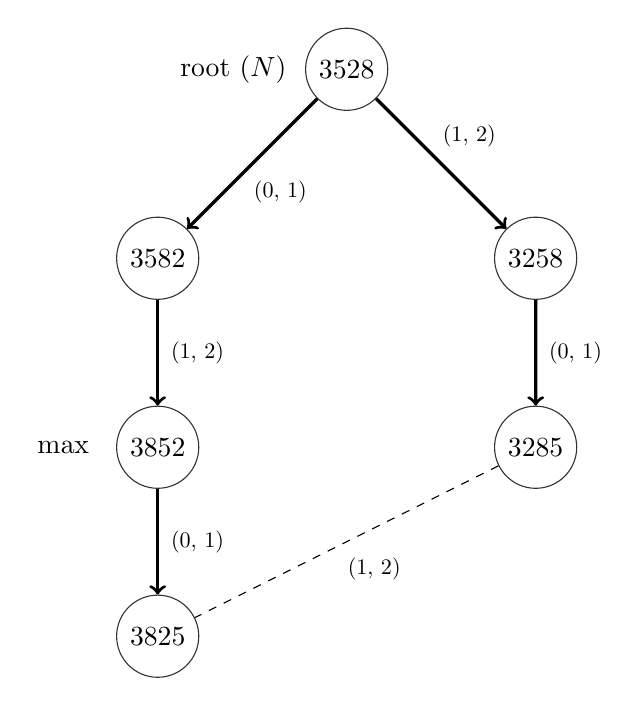
\begin{tikzpicture}
        [scale=.8,auto=left,every node/.style={circle,draw=black!80}]
            \node (n1)  at (3,9) {3528};
            \node (n2)  at (0,6) {3582};
            \node (n3)  at (6,6) {3258};
            \node (n4)  at (0,3) {3852};
            \node (n5)  at (6,3) {3285};
            \node (n6)  at (0,0) {3825};

        \foreach \from/\to/\name in {
            n1/n2/{(0, 1)},
            n1/n3/{(1, 2)},
            n2/n4/{(1, 2)},
            n3/n5/{(0, 1)},
            n4/n6/{(0, 1)}}
        \path[->,very thick] (\from) edge node[opacity=0,text opacity=1,scale=.8,draw=black!0] {\name} (\to);

        \node[style={rectangle,draw=black!0}] at (1.2, 9) {root ($N$)};
        \node[style={rectangle,draw=black!0}] at (-1.5, 3) {max};

        \path[-,dashed] (n5) edge node[opacity=0,text opacity=1,scale=.8,draw=black!0] {(1, 2)} (n6);
    \end{tikzpicture}
    \caption*{BFS Tree}
    \end{figure}

    So, the final answer given by the algorithm will be $(0,1), (1,2)$, i.e. $2$ exchanges in this order.
  }
  \subsection{Proof of Correctness}{
    I'll do the proof for this algorithm by 2 claims.
    \begin{claim}
      The above algorithm will give the path to the largest achievable number from the sequence $N$ under the restriction of exchange operations provided by $E$.
    \end{claim}
    \begin{proof}
      I will prove the above claim by contradiction.\newline
      Suppose the largest achievable number has the value $x$, the permutation of digits in the number $x$ are from the result of doing a sequence of exchange operations from the set $E$ (as given in the problem statement). \newline
      Since, we are considering $x$ is not the number we gain from the algorithm, so $2$ cases are possible. \newline
      \bold{Case I}:
      \begin{myenv}
        $x$ is not the largest achievable number which is a contradiction to our assumption as we already assumed that $x$ is the largest achievable number.
      \end{myenv}
      \bold{Case II}:
      \begin{myenv}
        The $Max$ value which we get from the algorithm is not the largest achievable number which means the value $x$ is either larger than $Max$ or $Max$ is not achievable by the set of exchange operations.\newline
        If we assume that $Max$ is not achievable by the given set of exchange operations, then it is a contradiction since the new vertex is generated from the old vertex by performing only the accepted exchange operations given by set $E$ (line $10$ of Algorithm $2$). \newline
        If we assume that $x$ is larger than $Max$ than it is also a contradiction, as if it was larger then the value of $Max$ would have been replaced by that of $x$ at line $16$ of Algorithm $2$.
      \end{myenv}
      Thus, by above $2$ cases of contradiction, it is proved that the number we finally get is actually the largest achievable number.
    \end{proof}
    \begin{claim}
      The above algorithm will give the minimum number of exchange operations to reach the largest achievable number.
    \end{claim}
    \begin{proof}
      The setup of the graph is such that each vertex is a possible permutation of the sequence and each edge will be an exchange operation from one vertex to other from the given set $E$. \newline
      So, the number of exchanges to reach the final number will be equal to the number of edges required to be travelled to reach the final node ($Max$). \newline
      The Algorithm implements the \bold{BFS} algorithm to calculate the shortest path from the initial node to the $Max$ node and since we get the shortest path, we will get the minimum number of exchanges possible, if there would have been less number of exchanges possible to reach the final node then the BFS algorithm would have given that as the shortest path. \newline
      Hence, the sequence of exchanges generated by the algorithm is the minimum number to reach the $Max$ node.
    \end{proof}
  }
  \subsection{Time Complexity Analysis}{
    The main portion of the code is the \bold{BFS} algorithm and the graph is generated while the algorithm is in play. \newline
    Since, the time complexity of \bold{BFS} algorithm is $O(V+E^{'})$, the maximum number of vertices possible is equal to the maximum number of permutations possible, thus, $V\leq10^{n}$. \newline
    Also, the max number of edges will be equal to half the product of number of elements in exchange operation set and number of vertices since every edge is created by application of exchange on a vertex. \newline
    Thus, time complexity is $O(|E| \times 10^{n})$.
  }
}
\end{document}
